\documentclass{article}
% \documentstyle[fullpage]{article}
\usepackage[utf8]{inputenc}
\usepackage{amsfonts}
\usepackage{amssymb}
\usepackage{geometry}
\usepackage{graphicx}

\geometry{a4paper, top = 25mm, bottom = 50mm, total = {6in, 8in}}

\renewcommand{\theenumi}{\alph{enumi}}
    
\title{COMP30026 Models of Computation \\ 
       Assignment 1 Submission}
\author{Liguo Chen\\Student ID: 851090}
\date{\today}

\begin{document}

\maketitle

\section*{Challenge 1}

\begin{enumerate}
    \item
    Let P(x,\ y) stand for `` x is a friend of y ''. If M is a friend of N, it's also true to say N is a friend of M. A person can be a friend of himself/herself.\\
    Let $D$ = \{Tom, Anna, Jack\} where Anna is a friend of Tom and Jack is a friend of Anna, but Tom and Jack don't know each other. Then,
    \begin{itemize}
    \setlength{\itemsep}{1pt}
        \item 
        $F$ is False as each of them are friends of themselves (P(x,\  x) is True for all x in the domain).
        \item
        $G$ is False when x is Tom, y is Anna and z is Jack. In this case, P(x,\ y) and P(y,\ z) are True, but P(x,\ z) is False. By the definition of implication, the formula is False.
        \item
        $G'$ is False when x is Tom, y is Anna and z is Tom. In this case, P(x,\ y) and P(y,\ z) are True, but $\neg P(x,\ z)$ is False. By the definition of implication, the formula is False.
        \item
        $G$ is False when x is Tom and y is Anna. In this case, P(x,\ y) is True, but $\neg P(y,\ x)$ is False. By the definition of implication, the formula is False.
    \end{itemize}
    As there exits interpretation that can make $F \vee G \vee G' \vee H$ False, the whole formula is not valid.
    \item
    Let P(x,\ y) = False and $D$ = $\mathbb{R}$
    \begin{itemize}
        \item 
        $F$ is True as P(x,\ x) is True for all x in the domain.
        \item
        $G'$ is True as the guard of the implication is False. By definition, the formula is True.
        \item
        $H$ is True as the guard of the implication is False. By definition, the formula is True. 
    \end{itemize}
    As there exits interpretation that can make $F \wedge G' \wedge H$ True, the whole formula is satisfiable.
    \item
    To prove $(F \wedge G) \Rightarrow H$ is valid, prove $\neg ((F \wedge G) \Rightarrow H)$ is unsatisfiable.\\
    % \begin{figure}
    %     \centering
    %     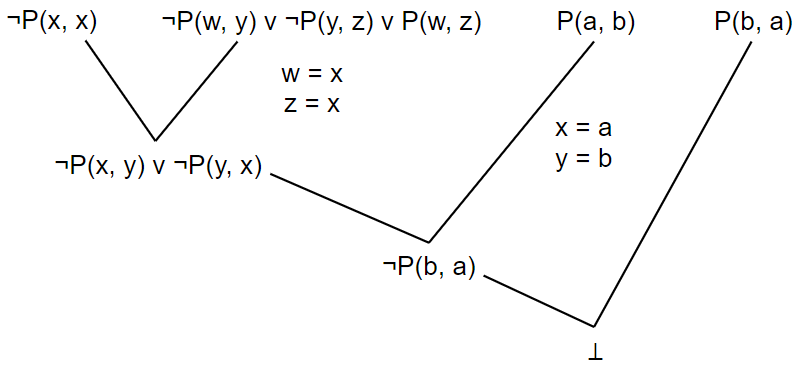
\includegraphics[width=10cm]{res}
    %     % \caption{Caption}
    %     % \label{fig:my_label}
    % \end{figure}\\
    Simplifying the formula $\neg ((F \wedge G) \Rightarrow H) \equiv F \wedge G \wedge \neg H$\\
    Change $F$, $G$ and $\neg H$ to clausal form:\\
    \hspace{1pt}\\
    \vspace{2pt}$F$: $\neg P(x,\ x)$\\
    %%%%%%%%%% for better readability
    $G$: $\forall x\ \forall y\ \forall z\ (P(x,\ y) \wedge P(y,\ z) \Rightarrow P(z,\ x))$\\
    \hspace*{4.5pt}$\equiv \forall x\ \forall y\ \forall z\ (\neg P(x,\ y) \vee \neg P(y,\ z) \vee P(x,\ z))$\\
    \vspace{2pt}\hspace*{4.5pt}$\equiv \neg P(x,\ y) \vee \neg P(y,\ z) \vee P(x,\ z)$\\
    % \vspace{5pt}\hspace*{4.5pt}$\equiv \neg P(u,\ u)\vee P(u,\ u)$\\
    %%%%%%%%%% for better readability
    $\neg H$: $\neg \forall x\ \forall y\ (P(x,\ y) \Rightarrow \neg P(y,\ x))$\\
    \hspace*{12.5pt}$\equiv\neg \forall x\ \forall y\ (\neg P(x,\ y) \vee \neg P(y,\ x))$\\
    \hspace*{12.5pt}$\equiv \exists x\ \exists y\ (P(x,\ y) \wedge P(y,\ x))$\\
    \vspace{10pt}\hspace*{12.5pt}$\leadsto P(a,\ b) \wedge P(b,\ a)$\\
    % \begin{enumerate}
    % \setlength{\itemsep}{-0.3ex}
    %     \item [$F$:] $\neg P(x,\ x)$
    %     \item [$G$:] $\neg P(u,\ u) \vee P(u,\ u)$
    %     \item [$H$:] $\neg P(s,\ t) \vee \neg P(t,\ s)$
    % \end{enumerate}
    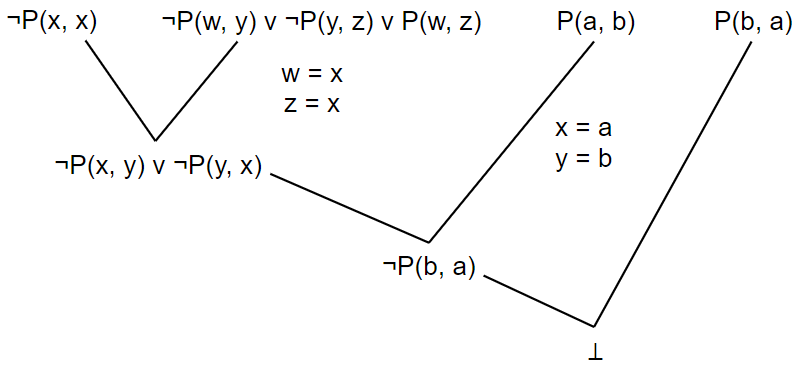
\includegraphics[width=11cm]{res}\\
    Therefore, $\neg ((F \wedge G) \Rightarrow H)$ is unsatisfiable, which means $(F \wedge G) \Rightarrow H$ is valid.
\end{enumerate}

\section*{Challenge 2}
\begin{enumerate}
    \item 
    $S_1$: $\forall x\ (J(x) \Rightarrow F(x))$  \\
    $S_2$: $\exists x\ (J(x) \wedge E(a,\ x))$  \\
    $S_3$: $\forall x\ (J(x) \Rightarrow (F(x) \wedge \forall y\ (P(y,\ x) \Rightarrow E(y,\ x)))) \Rightarrow V(x)$  \\
    $S_4$: $\forall x\ (J(x) \Rightarrow \neg\exists y\ (P(y,\ x))) \Rightarrow V(x)$
    
    \item
    $S_1$: $\neg J(x) \vee F(x)$\\
    %%%%%%%%%% for better readability
    $S_2$: $J(b) \wedge E(a, b)$\\
    %%%%%%%%%% for better readability
    $S_3$: $\forall x\ (J(x) \Rightarrow (F(x) \wedge \forall y\ (P(y,\ x) \Rightarrow E(y,\ x)))) \Rightarrow V(x)$\\
    \hspace*{7.5pt}$\equiv \forall x\ \neg(\neg J(x) \vee (F(x) \wedge \forall y\ (\neg P(y,\ x) \vee E(y,\ x)))) \vee V(x)$\\
    \hspace*{7.5pt}$\equiv \forall x\ (J(x) \wedge (\neg F(x) \vee \exists y\ (P(y,\ x) \wedge \neg E(y,\ x) ))) \vee V(x)$\\
    \hspace*{7.5pt}$\leadsto \forall x\ (J(x) \wedge (\neg F(x) \vee (P(f(x),\ x) \wedge \neg E(f(x),\ x)))) \vee V(x)$\\
    \hspace*{7.5pt}$\equiv (J(x) \wedge (\neg F(x) \vee P(f(x),\ x)) \wedge (\neg F(x) \vee \neg E(f(x),\ x))) \vee V(x)$\\
    \hspace*{7.5pt}$\equiv (J(x) \vee V(x)) \wedge (\neg F(x) \vee P(f(x),\ x) \vee V(x)) \wedge (\neg F(x) \vee \neg E(f(x),\ x) \vee V(x))$
        % \begin{enumerate}
        %     \item [$S_1$:] $\neg J(x) \vee F(x)$\ (or $\{J(x),\ F(x)\}$)
        %     \item [$S_2$:] $J(b) \wedge E(a, b)$\ (or $\{\{J(b)\},\ \{E(a, b)\}\}$)
        %     \item [$S_3$:] $\forall x\ (J(x) \Rightarrow (F(x) \wedge \forall y\ (P(y,\ x) \wedge (E(y,\ x))))) \Rightarrow V(x)$\\
        %     dd
        % \end{enumerate}
    
    \item 
    $\neg S_4$: $\neg (\forall x\ (J(x) \Rightarrow \neg\exists y\ (P(y,\ x))) \Rightarrow V(x))$\\
    \hspace*{14pt}$\equiv \neg(\forall x\ \neg(\neg J(x) \vee \neg\exists y (P(y,\ x))) \vee V(x))$\\
    \hspace*{14pt}$\equiv \exists x\ (\neg J(x) \vee \forall y\ (\neg P(y,\ x))) \wedge \neg V(x)$\\
    \hspace*{12.5pt}$\leadsto (\neg J(c) \vee \forall y\ (\neg P(y,\ c))) \wedge \neg V(c)$\\
    \hspace*{14pt}$\equiv (\neg J(c) \vee \neg P(y,\ c)) \wedge \neg V(c)$
    \item
    \hspace{1pt}\\
    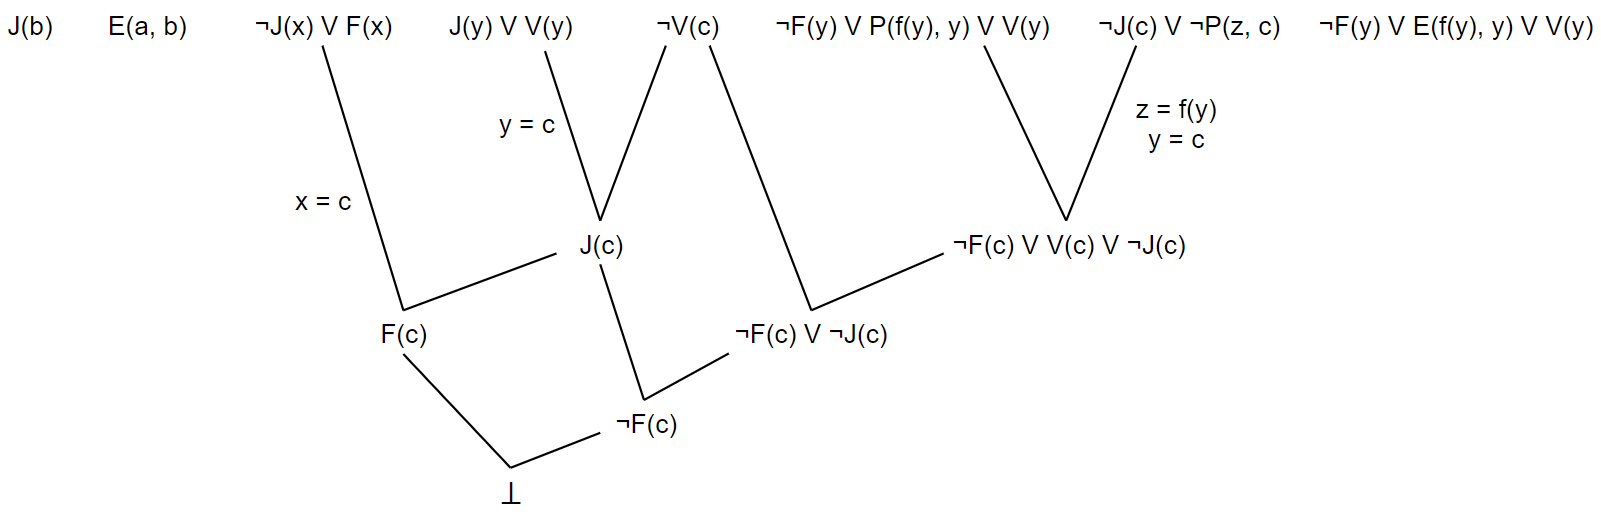
\includegraphics[width=15cm, height=5cm]{res2}
\end{enumerate}

\section*{Challenge 3}
 \begin{enumerate}
 \setlength{\itemsep}{1ex}
     \item
      \hspace{1pt}\\
         \begin{tabular}{|c|c|c|}
             \hline
             $b_1$ & $b_2$ & $(\neg b_1, b_1 \oplus b_2)$ \\
             \hline
             0 & 0 & (1, 0) \\
             \hline
             0 & 1 & (1, 1) \\
             \hline
             1 & 0 & (0, 1) \\
             \hline
             1 & 1 & (0, 0) \\
             \hline 
         \end{tabular}
         
        With different inputs, the function produces different outputs.\\Therefore, it is reversible.
     \item
     \hspace{1pt}\\
         \begin{tabular}{|c|c|c|c|}
              \hline
              $b_1$ & $b_2$ & $b_3$ & $(b_1 \oplus b_2, b_2 \oplus b_3, b_3 \oplus b_1)$ \\
              \hline
              0 & 0 & 0 & (0, 0, 0) \\
              \hline
              0 & 0 & 1 & (0, 1, 1) \\
              \hline
              0 & 1 & 0 & (1, 1, 0) \\
              \hline
              0 & 1 & 1 & (1, 0, 1) \\
              \hline
              1 & 0 & 0 & (1, 0, 1) \\
              \hline
              1 & 0 & 1 & (1, 1, 0) \\
              \hline
              1 & 1 & 0 & (0, 1, 1) \\
              \hline
              1 & 1 & 1 & (0, 0, 0) \\
              \hline
         \end{tabular}
         
         Row 1 and 8 are the same.\\
         Row 2 and 7 are the same.\\
         Row 3 and 6 are the same.\\
         Row 4 and 5 are the same.\\
         With different inputs, the function produces same outputs.\\
         Therefore, it is not reversible.
     \item
     \hspace{1pt}\\
     \begin{tabular}{|c|c|c|c|}
              \hline
              $b_1$ & $b_2$ & $b_3$ & $(b_1 \oplus b_3, \neg b_3, b_1 \oplus b_2)$ \\
              \hline
              0 & 0 & 0 & (0, 1, 0) \\
              \hline
              0 & 0 & 1 & (1, 0, 0) \\
              \hline
              0 & 1 & 0 & (0, 1, 1) \\
              \hline
              0 & 1 & 1 & (1, 0, 1) \\
              \hline
              1 & 0 & 0 & (1, 1, 1) \\
              \hline
              1 & 0 & 1 & (0, 0, 1) \\
              \hline
              1 & 1 & 0 & (1, 1, 0) \\
              \hline
              1 & 1 & 1 & (0, 0, 0) \\
              \hline
         \end{tabular}
         
         With different inputs, the function produces different outputs.\\Therefore, it is reversible.
     \item
     The total number of distinct bit strings with length n is $2^n$. A reversible function can be thought of as a mapping from the input string to one of the remaining strings (those that are not bound by any mapping). As these strings are all different, this is like permutation of the $2^n$ bit strings (swapping any two will produce a different result). So, the total number of reversible functions is $(2^n)!$. When reversibility is not required, an input string can be mapped to any of the $2^n$ strings, doesn't matter if it's bound or not. Hence, there will be $2^n$ different mappings for each input string, and the total number for all input strings is $(2^n)^{2^n}$. Therefore, the fraction of reversible function is ${(2^n)!}\ /\ {(2^n)^{2^n}}$.
 \end{enumerate}

\end{document}
